\section{Considerações iniciais}

Segundo o relatório técnico \citeonline{MineralCommodity2007}, o concreto é atualmente considerado o material estrutural mais utilizado no mundo, ficando em segundo lugar em materiais gerais, perdendo apenas para a água. 
Os cálculos apresentados por \citeonline{Gagg2014} relatam que há o dobro de concreto sendo utilizado em construções do que a soma da utilização de aço, alumínio, madeira e plástico, com isso podendo ser encontrado na maioria das categorias de construções, desde casas de alvenaria até pontes, usinas e plataformas de extração petrolíferas \cite{Lima2014}.

Nessa linha de raciocínio, é necessário entender o básico de seus conceitos e sua contextualização na problemática desta pesquisa. Logo, neste capítulo, serão abordados os conceitos de concreto, sua aplicação em OAE's, suas variações de aplicações, o limite de sua vida útil e patologias.

\section{Conceitos gerais}

Por mais comum que seja, ainda há uma falta de conhecimento sobre o que realmente é o concreto, e qual é a diferença entre ele é o cimento, já que ambos termos são comumente usados de forma conjunta \cite{Gagg2014}. 
O concreto é o resultado de uma mistura de diversos materiais, sendo o principal destes o cimento, que é o material aglutinante deste compósito, agrupando todos os materiais que compõem o concreto. \cite{allen2019fundamentals}.
A receita dessa mistura pode ser modificada, porém o padrão é a mistura de água, cimento, agregados miúdos como areia, e agregados graúdos como cascalho, aditivos e adições. 
A modificação da quantidade de cada elemento pode fazer com que o concreto fabricado obtenha características diferentes, tornando o concreto um material versátil capaz de se adequar a diferentes tipos de estruturas, como pilares, paredes, piso, entre outros \cite{Gagg2014}.

Dentre essas características, a que mais se destaca é de resistência à compressão, sendo a quantidade de força de compressão resistida pelo concreto, geralmente medido em \sigla{MPa}{Megapascal} \cite{pinheiro2007fundamentos}. 
Para cada tipo de estrutura há a necessidade de uma certa resistência para que se tenha força o suficiente para sustentar tal estrutura \cite{izharcomparison}.


\section{Concreto armado}

O concreto armado é um material que emprega o concreto tradicional e uma adição de barras de aço, onde ambos se complementam para resistir respectivamente às forças de compressão e tração \cite{Lima2014}. 
Essas barras de aço, chamadas de armadura do concreto, oferecem ao concreto a resistência necessária para combater esforços de tração, necessária em todas as peças estruturais que formam edificações, pontes e outras estruturas \cite{pinheiro2010estruturas}.

\section{Obra de arte especial}

De acordo com a definição dada pelo engenheiro civil e pesquisador \citeonline{Ciro2014}, \sigla{OAE}{Obra de Arte Especial} é uma construção estrutural com a finalidade de transpor grandes obstáculos, tais como rios, desníveis, porções urbanas, entre outros; dessa forma, se configura como OAE estruturas como pontes quando construídas sobre níveis de água, como viadutos quando sobre avenidas ou espaços secos, e como túneis em casos abaixo da superfície.

No Brasil, o principal órgão regulador dessas estruturas, a nível federal, é o \sigla{DNIT}{Departamento Nacional de Infraestrutura de Transporte}, autarquia responsável por implementar a política de infraestrutura de transportes terrestres e aquaviários,
estabelecendo as regras de construção e monitoramento que devem ser seguidas pelos construtores \cite{dnitdados}.

Como dito anteriormente, o concreto, principalmente o concreto armado, possui uma incrível resistência á compressão, fazendo-o uma ótima escolha como elemento principal na construção das OAE's, ainda mais quando comparado seu custo operacional e disponibilidade no mercado \cite{santos2008armaccao}. 


No entanto, assim como acontece com todo material estrutural, o concreto está sujeito a diversas formas de deterioração, que podem ser causadas tanto pelo uso quanto por ações naturais \cite{santos2008armaccao}.
Portanto, se faz necessário estudar métodos que ajudem com a manutenção dessas estruturas, principalmente a de concreto, por ser a mais utilizada \cite{santos2008armaccao}.

Percebendo essa situação, o DNIT torna obrigatório o monitoramento das OAE's no mínimo a cada dois anos e sendo obrigatório a presença de inspetores qualificados e inspetores auxiliares.
A vistoria consiste em um processo demorado da criação de um relatório que envolve a observação de toda a OAE, captura de evidências visuais como fotos ou vídeos e descrição por escrito da situação da OAE, de suas falhas e expectativa para os próximos anos \cite{dnit2004}.

\section{Falhas estruturais}

De acordo com o conceito relatado por \citeonline{afonso2021}, as falhas estruturais ocorrem quando um componente ou até mesmo toda a estrutura perde a capacidade de uso estabelecida no projeto, e essas falhas podem ser classificadas de acordo com o fator que as desencadeou.
Em especial para esta pesquisa, as falhas causadas por conta de fraturas são chamadas de falha frágil sendo geralmente resultante de danos acumulados, que com o tempo fazem com que o material estrutural perca sua resistência, dessa forma também sendo configurado como um dano progressivo \cite{anneLink2016}.

 Segundo \citeonline{cremonini1988incidencia}, o concreto é de fato um material com uma resistência muito alta, tanto em questão de cargas quanto em agressões ambientais, porém essa resistência pode vir a ruir, comprometendo sua capacidade de suportar os empenhos solicitados. 
 Ao fazer o estudo dos causadores dessa perda de resistência, a engenharia emprega o termo patologia aos tipos de causas e origens de tais problemas \cite{cremonini1988incidencia}.
 
 À vista disso, é imprescindível  que se tenha a realização de estudos sobre tais patologias e como evitá-las. Algumas das patologias mais comuns \cite{statera} encontradas são fissuras, corrosão de armadura e falhas de Concretagem.

\subsection{Fissuras}

A presença de fissuras em estruturas que empregam concreto armado pode acarretar em graves problemas estruturais e representa um sério indicador de degradação do estado de conservação.
Nos piores casos, a falta de manutenção apropriada faz com que toda a estrutura se comprometa, perdendo todo seu caráter estético, social, econômico, ademais dos riscos de segurança ao usuário \cite{santos2014patologia}.

Assim, é inegável que a ocorrência de fissuras é um problema de grande importância, que afeta áreas tão diversas, desde o campo econômico até mesmo questões psicológicas já que a presença de fissuras pode gerar preocupação e insegurança, principalmente em edifícios de grande porte \cite{andrade1998durabilidade}.
Por conta disso, é necessário entender suas causas e origens para descobrir então suas consequências e as remediações necessárias de modo a recuperar e estender sua vida útil \cite{de1998patologia}.

Existem variados tipos de fissuras que podem acontecer em estruturas de concreto armado, sendo que cada fator implica em diferentes tipos de fissuras \cite{nakamura2007}. 
A falta de umidade no concreto provoca o aparecimento de várias aberturas lineares, esse tipo de fissura é chamado de fissura por retração. 
Quando é adicionado mais carga do que o calculado em uma estrutura pode acontecer as chamadas fissuras de sobrecarga que costumam ser graves e requerem manutenção urgente. 
Em estruturas que envolvem a combinação de diferentes materiais, pode ocorrer que esses materiais não reajam da mesma maneira às forças de dilatação.

Um exemplo desse problema é a combinação de de concreto, tijolos, pedras ou outros elementos similares para formar a chamada estrutura de alvenaria, onde acontece a chamada fissuras higro-térmicas causada pela combinação de movimentos térmicos e variações na umidade dos materiais de construção \cite{nakamura2007}.

Por conta desses e de vários outros motivos, o DNIT apresenta uma série de regras e de instruções para a realização da manutenção de cada patologia e cada material utilizado em OAE's. Exemplos dessa patologia podem ser vistas em \autoref{fig:fissuras}.

\begin{figure}[htb]
\centering
\caption{Exemplos de fissuras em estruturas de concreto.}
    \begin{subfigure}{.5\textwidth}
      \centering
      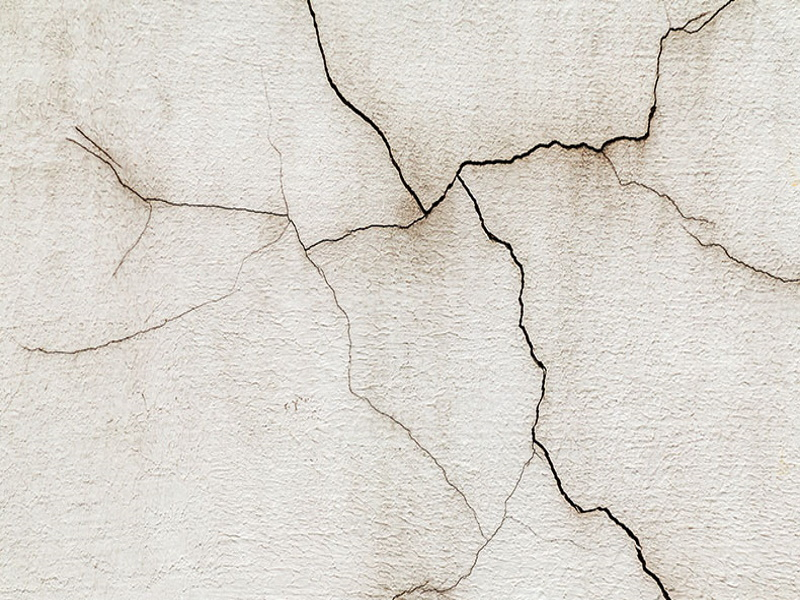
\includegraphics[width=.8\linewidth]{images/mapa_da_obra_img_fissura.jpg}
      % \caption{A subfigure}
      \label{fig:fissura01}
      \fdireta{fig:fissura01}
    \end{subfigure}%
    \begin{subfigure}{.5\textwidth}
      \centering
      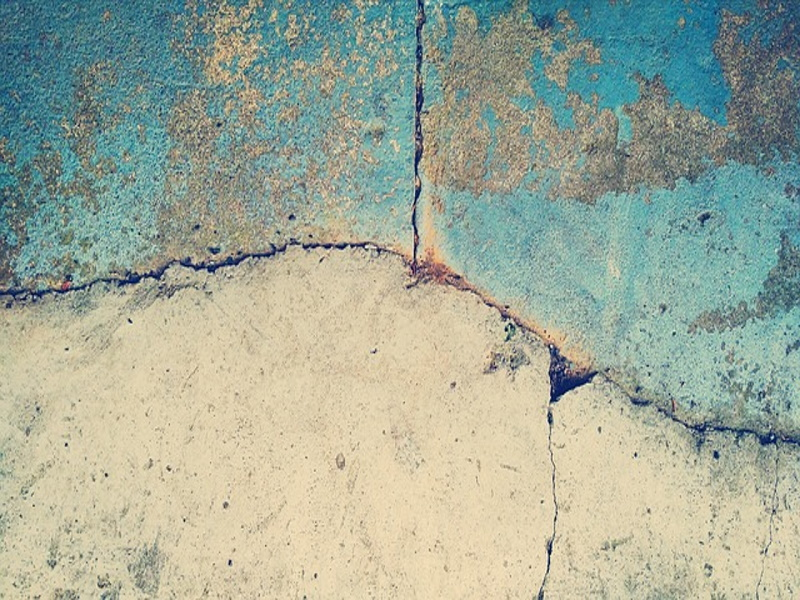
\includegraphics[width=.8\linewidth]{images/tudo_construcao_fissura02.jpg}
      % \caption{A subfigure}
      \label{fig:fissura02}
      \fdireta{fig:fissura02}
    \end{subfigure}


\label{fig:fissuras}
\end{figure}

\subsection{Corrosão de armadura}

O concreto armado é um excelente material estrutural, pois sua composição permite que um dos materiais possa remediar os problemas apresentados pelos outros \cite{pinheiro2010estruturas}. 
Um exemplo disso é a forte alcalinidade do concreto, que atua na proteção da armadura contra a corrosão \cite{pinheiro2010estruturas}.
Porém, uma possível patologia, que geralmente acontece pela falha durante a concretagem, ou por erros de cálculo para determinar a espessura do concreto, podem resultar na exposição da armadura, fazendo com que a exposição ao dióxido de carbono do ambiente faça a corrosão acontecer \cite{statera}. 
No caso de certas OAE's, como pontes, existem uma maior quantidade de agentes agressivos, como em zonas marítimas onde há o vento que carrega partículas de sal \cite{statera}.

Além de ser a patologia mais usual nas estruturas de concreto armado, a corrosão de armadura também é uma das mais perigosas, sendo considerado uma anomalia grave cujo eventual produto pode vir a ser o colapso total da estrutura \cite{tecnosil_2017}. 
Posterior ao início dessa patologia, se não houver tratamento e manutenção, a corrosão manifesta uma progressão constante e ininterrupta em todos os casos \cite{tecnosil_2017}.
A influência dessa patologia em estruturas de concreto pode ser observada na \autoref{fig:cor_armd}.

\begin{figure}[htb]
\centering
\caption{Exemplos de corrosão de armadura em estruturas de concreto.}
    \begin{subfigure}{.5\textwidth}
      \centering
      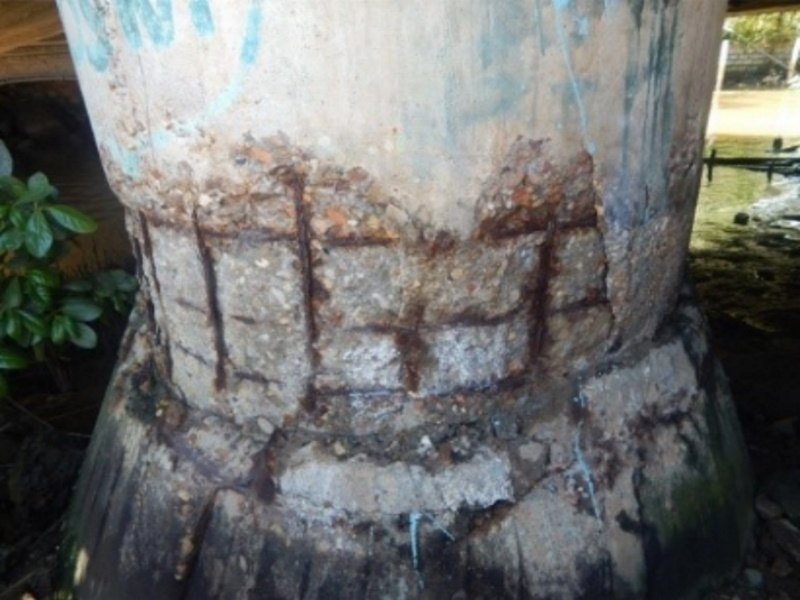
\includegraphics[width=.8\linewidth]{images/corrosao_armadura01.jpg}
      % \caption{A subfigure}
      \label{fig:corrosao01}
      \fdireta{antuneslevantamento}
    \end{subfigure}%
    \begin{subfigure}{.5\textwidth}
      \centering
      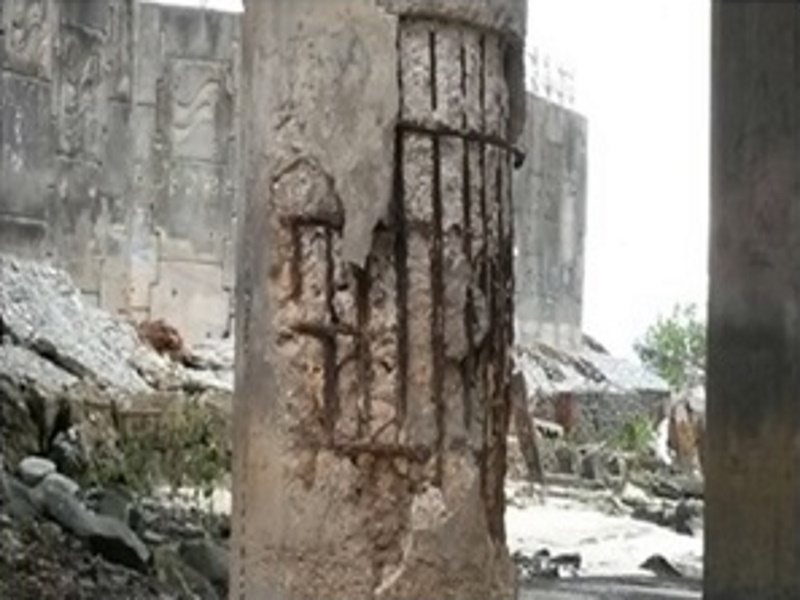
\includegraphics[width=.8\linewidth]{images/corrosao02.jpg}
      % \caption{A subfigure}
      \label{fig:corrosao02}
      \fdireta{fig:corr02}
    \end{subfigure}

\label{fig:cor_armd}
\end{figure}
    
\subsection{Falhas de concretagem}
    
As falhas de concretagem denominam as irregularidades que ocorrem no período do processo de concretagem por conta de erros de posicionamento e compactação do concreto \cite{statera}.
Segundo \cite{zhou2020concrete}, projetos deficientes, de execução mal feitas são os principais responsáveis pelo surgimento de patologias.

Para reprimir que tais erros ocorram, há uma série de diretrizes que cada projeto deve executar.
No caso de OAE's o órgão emissor dessas diretrizes é o DNIT. 
Contudo, segundo \citeonline{tecnhe_2010}, no contexto atual da construção civil, não estão sendo seguidos os prazos sugeridos para cada etapa construtiva.
Diminuir o tempo de cada etapa resulta também em menos tempo para planejar e projetar as características da obra e de seus componentes.

\section{Problemas/prejuízos causados pelas fissuras}

Embora não apresente problemas sérios diretamente, as fissuras representam o sinal inicial de que um problema sério pode vir a acontecer \cite{alani2014integrated}, por conta disso o DNIT exige que aconteça regularmente uma inspeção \cite{dnit2004}.
Uma inspeção realizada da forma correta consegue produzir várias informações do estado atual da estrutura através da
medição de grandezas físicas, como acelerações, deformações, e/ou deslocamentos.

O problema é que o método tradicional de inspeção, que é o manual, pode ser considerado um trabalho extensivo, custoso, e possivelmente perigoso, além de necessitar da contratação de técnicos capacitados e de confiança \cite{adhikari2014image}.
Outro grande custo é o carecimento de certas ferramentas e equipamentos, em especial em lugares de difícil acesso onde é necessário a utilização de certos veículos especializados, como caminhão com cesta elevatória \cite{dorafshan2018bridge}.
Há ainda o fator do descontentamento gerado ao público, pois geralmente há a necessidade de no mínimo limitar o acesso à OAE, o que também causa custos de forma indireta \cite{catbas2018vision}.

\section{Enfoque computacional para solucionar o problema}

Com o objetivo de auxiliar o serviço de manutenção e monitoramento, vários autores buscam desenvolver novas ferramentas e métodos como alternativas para abordar o problema em questão.
Tais autores concordam que as melhores soluções possíveis estão dentro do campo computacional e portanto se faz necessário o estudo com enfoque computacional dentro da engenharia.

\subsection{Sensoriamento}

Uma das primeiras soluções encontradas foi a de utilizar redes de sensores a fim de que extraiam  dados da estrutura em tempo real, para que o técnico responsável tivesse acesso a tais informações sempre que requerido \cite{spencer2019advances}.
Embora seja uma alternativa recomendável, esta alternativa continua sendo problemática devido aos altos custos envolvidos, mesmo com as evoluções tecnológicas ocorridas até os dias atuais \cite{Zhuang2022}.
Entre os desafios enfrentados se destacam: realizar a instalação da fiação de cabos por toda a estrutura, transmissão e geração de energia para sustentar a cadeia de sensores, transferência de dados entre si e para um sistema receptor, calibração regular dos sensores \cite{catbas2018vision}.

\subsection{Visão computacional}

Com o passar do tempo, os métodos baseados em visão computacional ganharam maior notoriedade por conta de seus resultados em identificação, classificação e localização de objetos dentro de imagens.
Em razão disso \citeonline{webb2015categories} apresentam a visão computacional como uma possibilidade para ser utilizada na engenharia civil, em específico no âmbito de inspeções e monitoramento.

Ao utilizar imagens e vídeos como dados de análise para o computador é possível obter as informações necessárias para o monitoramento \cite{spencer2019advances} sem a necessidade do contato direto humano, evidentemente, sendo essa sua maior vantagem \cite{catbas2018vision}.

Uma outra vantagem da visão computacional é a flexibilidade de equipamento, já que hoje até mesmo as câmeras de telefones conseguem registrar imagens de alta qualidade, contudo seja recomendado equipamentos como câmeras de alta performance ou até drones \cite{dorafshan2018bridge}.
Atualmente, os drones têm conquistado espaço em vários ambientes profissionais, sendo considerado uma ferramenta eficiente, contributiva e uma alta relação de custo-benefício \cite{zoubir2021crack}. 

Com essas tecnologias de visão computacional citadas e um investimento mínimo, é possível até mesmo implementar um sistema automatizado de coleta das imagens. 
Entretanto, mesmo com a automatização da captura de imagens, seja através de câmeras estacionárias, drones ou outro método, ainda há a parte mais tediosa e custosa em questão de tempo, que é a de um técnico especialista realizar a análise interpretativa dos dados coletados \cite{zoubir2021crack}, essa etapa, porém, pode ser também automatizada a partir de métodos computacionais.

\subsection{Métodos matemáticos}

Durante o começo das pesquisas de visão computacional, as principais ferramentas a serem utilizadas para detectar problemas em estruturas eram caracterizadas como heurísticas. 
Normalmente essas heurísticas eram executadas com a aplicação de limiar ou com a criação de filtros específicos \cite{spencer2019advances}, que posteriormente poderiam até ser calculados utilizando aprendizagem de máquina.

Os tipos de filtros mais comuns utilizados em trabalhos recentes para a segmentação de imagens são os detectores de bordas. 
A partir de alguma premissa especificada pelo usuário, esses algoritmos buscam em uma imagem uma série de pontos onde existam mudanças bruscas que interligados configuram algum objeto, realizando, assim, a segmentação da imagem \cite{ziou1998edge}.

Em um dos primeiros trabalhos específicos da área, \citeonline{abdel2003analysis} utilizam os detectores de borda \textit{Sobel} e \textit{Canny} e as transformadas de \textit{Fourier} e \textit{Fast Haar} como gradiente para detecção de borda em 50 fotos adquiridas a partir de câmeras fotográficas e conseguindo uma acurácia dividida entre 86 e 64\% dentre seus métodos, sendo a transformada de \textit{Fast Haar} a que gerou o melhor resultado, porém sendo ainda necessário a interpretação de um usuário para separar o que realmente são fissuras dos erros causados pela textura. 

No trabalho de \citeonline{jahanshahi2009survey}, é realizada uma comparação entre o método de detecção de borda e a união de operações morfológicas. 
O estudo descreve de forma detalhada os cálculos utilizados em cada um desses métodos.
Os cálculos utilizados para o método de detecção de borda incluem: cálculos de derivadas de autovalores e autovetores, gradientes, filtro Gaussiano e Laplaciano, transformadas de \textit{Fast Haar}, limiarização baseada em mediana e uma pequena camada de rede neural de uma camada para caracterizar os objetos gerados. 
Com isso, é obtida uma precisão de 71,5\%, que o autor compara ao trabalho anterior citado devido à similaridade. 
Também é explicado que a diferença de resultados ocorre principalmente devido à mudança da direção da luz ao longo do dia \cite{abdel2003analysis}.
Já o método de operações morfológicas envolve a manipulação de uma matriz de valores de escala de cinza, onde os processos morfológicos mais básicos, como a dilatação e a erosão, são aplicados. 
Através da combinação desses processos, diversas operações podem ser realizadas, como abertura, fechamento, gradiente morfológico, \textit{bottom-hat} e \textit{top-hat}. 
No entanto, é necessário utilizar um elemento estruturante de tamanho adequado para cada tipo de imagem, o que pode tornar a abordagem menos flexível. 
Embora o autor não tenha informado a porcentagem de acurácia, ele considera essa abordagem mais efetiva do que o detector de bordas, pois gera menos ruído.

Finalmente, em seu estudo, \citeonline{dorafshan2019benchmarking} realizaram uma comparação da eficiência, precisão e tempo de processamento de quatro filtros distintos para a detecção de bordas no domínio espacial e dois filtros no domínio de frequência. 
A base de dados utilizada para a análise foi composta por 50 imagens de concreto em condições saudáveis e outras 50 imagens com a presença de fissuras, ambas coletadas por meio de drones.
Inicialmente, o método empregado realiza a conversão da imagem para níveis de cinza com uma ponderação maior na cor verde, uma ponderação média na cor vermelha e uma ponderação menor na cor azul. 
Em seguida, o filtro selecionado é aplicado a esta nova imagem, utilizando uma matriz de valores que são convoluídos na operação. 
Os filtros avaliados incluem \textit{Roberts}, \textit{Prewitt}, \textit{Sobel} e \textit{Laplacian of Gaussian} no domínio espacial, e \textit{Butterworth} e \textit{Gaussian} no domínio de frequência.
No domínio de frequência, é preciso converter a imagem do domínio espacial para o domínio de frequência usando a transformada rápida de Fourier (\textit{Fast Fourier Transform}). 
Depois de aplicar cada filtro, é realizada uma melhoria na imagem resultante, principalmente através da normalização com base na média e no desvio padrão, e ajuste de brilho para melhorar a visibilidade das bordas.
Por fim, a imagem é segmentada, resultando em uma nova imagem binária que mostra positivamente os locais onde existem rachaduras. 
Esse processo é realizado através do método de \textit{Otsu}, que encontra um limiar de corte adequado.
Para avaliar a eficácia do método, um inspetor revisou as imagens e classificou manualmente cada uma delas, alcançando uma acurácia de 100\%.
Em seguida, comparou-se os resultados dos filtros com os rótulos do inspetor, obtendo-se uma acurácia de 77\% a 92\%, precisão de 82\% a 88\%, e um tempo de processamento variando de 1.18 a 1.92 segundos. 
O filtro \textit{Laplacian of Gaussian} obteve os melhores resultados, com 92\% de acurácia, 88\% de precisão e tempo de processamento de 1.18 segundos.

\subsection{Deep learning}

Com o avanço da tecnologia computacional e o desenvolvimento de algoritmos mais avançados, as redes neurais profundas de convolução se tornaram uma abordagem promissora para a classificação e segmentação de imagens. 
De fato, estudos recentes demonstraram que esses métodos superam outras técnicas de aprendizado de máquina nessa área \cite{zhou2020concrete}. 
Além disso, quando aplicados à engenharia, esses métodos têm o potencial de alcançar resultados sem precedentes \cite{qiao2021computer}.

Exemplos de como as redes neurais profundas de convolução têm sido utilizadas em detecção de fissuras podem ser encontrados em diversos estudos, como em \citeonline{dorafshan2018comparison}, que comparou diferentes métodos de processamento de imagem com o método baseado em rede convolucional de aprendizado de máquina.
E de forma correlacionada ao objetivo desta monografia, há exemplos como os autores \citeonline{Zhang2017} e \citeonline{zhang2018deep}, que desenvolveram modelos específicos para detecção de fissuras usando redes convolucionais. 
Além disso, estudos como \citeonline{qiao2021computer} demonstraram resultados promissores ao aplicar arquiteturas conhecidas de redes convolucionais na detecção de fissuras em imagens de concreto.

Com o crescente interesse em soluções de alta precisão em detecção e classificação de fissuras em estruturas de concreto, os modelos baseados em \textit{deep learning} têm se tornado cada vez mais requisitados na área. Autores como \citeonline{zoubir2021crack}, \citeonline{ichi2021sdnet2021} e \citeonline{maguire2018sdnet2018} se concentram em apresentar avanços na coleta de dados, especialmente imagens, para auxiliar no treinamento dos modelos de \textit{deep learning}.

